% L8b student companion deck.
%
% The frame order mirrors the lecture notebook so students can take notes while
% the instructor works through the notebook. The disclaimer is intentionally
% slide 2, by instructor preference.
%
% Notation follows the lecture notebook: standalone premiums
% C_0 and P_0 (matching L9a and L11a), payoff functions h_c/h_p (matching L9a),
% and leg quantities i, h_i, P_i, H_C, Pi_C, theta_i, n_i (matching L10b).
% Composite totals are per share; the deliverable q_i converts to account
% dollars and is applied per leg, inside the account-dollar sum, because the
% legs need not share a deliverable.
\documentclass[aspectratio=169,11pt]{beamer}
\usepackage{vnslides}

\newcommand{\E}{\mathbb{E}}
\newcommand{\R}{\mathbb{R}}
\newcommand{\N}{\mathbb{N}}
\newcommand{\ST}{S_{T}}
\newcommand{\CC}{\mathcal{C}}
\newcommand{\hc}{h_{c}}
\newcommand{\hp}{h_{p}}
\newcommand{\PiC}{\Pi_{\CC}}
\newcommand{\HC}{H_{\CC}}

\title{\texorpdfstring{{\vnheavy L8b}}{L8b}: Option Contracts: Call and Put Payoff and Profit}
\subtitle{CHEME 5660 Cornell University}
\author{Copyright Jeffrey Varner 2026. All Rights Reserved}

\begin{document}

\vntitlepage

\begin{frame}{Disclaimer and Risks}
  \vspace{0.6em}
  \textbf{\ink{Training only.}} This content is for training and informational
  purposes only. The teaching team does not make, give, or endorse any offer or
  solicitation to buy or sell securities or derivative products, or provide
  investment or trading advice or strategy.

  \vspace{1.1em}
  \textbf{\ink{Risk.}} Trading involves risk and is generally not recommended for
  those with limited resources, experience, or a low risk tolerance. Past
  performance does not guarantee future success.

  \vspace{1.1em}
  \textbf{\ink{Responsibility.}} You are responsible for your investment decisions
  based on your financial circumstances, objectives, risk tolerance, and
  liquidity needs.
\end{frame}

\begin{frame}{Objectives for Today}
  Today opens Unit 3. Units 1 and 2 modeled assets we hold directly; a
  \hilite{derivative} is instead a contract whose cash flows are a function of
  someone else's price. We read the contract, compute what it pays at
  expiration, and keep what the contract promises separate from what the
  investor earns.

  \vspace{0.5em}
  {\large\textbf{\ink{Today's concepts}}}
  \vspace{0.2em}
  \begin{itemize}\setlength{\itemsep}{0.4em}
    \item \hilite{Read an option contract}: underlying, strike $K$, expiration
      $T$, exercise style, deliverable $q$, direction $\theta$, and the premium:
      which are contractual, which is quoted.
    \item \hilite{Separate payoff from profit}: the expiration payoff of all four
      positions, the premium adjustment and the convention it hides, the
      breakeven prices, and the maximum profit and loss of each.
    \item \hilite{Compose positions}: a strategy as a signed sum of legs, with a
      corner at each strike where the legs do not cancel and an offset set by
      the net debit or credit.
  \end{itemize}
\end{frame}

\begin{frame}{Lectures and Examples}
  \vspace{0.3em}
  {\normalsize\textbf{\ink{Lecture:}}\par
  \dimmed{CHEME-5660-L8b-Lecture-IntroductionToDerivativesContracts-Fall-2026.ipynb}}

  \vspace{0.6em}
  {\normalsize\textbf{\ink{Example 1:}}\par
  \dimmed{CHEME-5660-L8b-Example-SingleContractPayoffProfit-Fall-2026.ipynb}}

  \vspace{0.6em}
  {\normalsize\textbf{\ink{Example 2:}}\par
  \dimmed{CHEME-5660-L8b-Example-CompositeContractsPL-Fall-2026.ipynb}}

  \vspace{0.5em}
  The first example builds all four single-contract positions from a real
  options chain, sweeps the full domain $\ST\geq0$, converts per-share
  quantities to per-contract dollars, and verifies every breakeven and bound
  numerically; the second combines signed legs into vertical spreads,
  straddles, and strangles.
\end{frame}

% ==== concept review =========================================
\begin{frame}{Concept Review: From Assets to Contracts Written on Assets}
  Units 1 and 2 priced and allocated assets we hold \hilite{directly}: Treasury
  cash flows (L2a, L2b), equity growth rates (L3a, L4b), and portfolios built
  from them (L5b through L7b).

  \vspace{0.4em}
  \textbf{\ink{Carried forward:}} the price of the underlying. Let $S_t\geq0$ be
  that price in USD/share at time $t$, so $S_0$ is today and $\ST$ is expiration.
  \begin{itemize}\setlength{\itemsep}{0.3em}
    \item \hilite{The payoff is contractual, not statistical}: given $\ST$, what
      the contract pays is a formula written into it. No estimation enters that
      step. Uncertainty enters only through $\ST$.
    \item \hilite{The two sides are not symmetric}: one counterparty holds a
      right, the other carries an obligation. The premium is the price of that
      asymmetry, and it is paid whether or not the right is ever used.
  \end{itemize}
\end{frame}

% ==== what is a derivative ===================================
\begin{frame}{What Is a Derivative?}
  A \hilite{derivative} is a contract whose cash flows depend on an underlying
  quantity: an equity price, a rate, a currency, a commodity, an index, or a
  credit event. The families differ in who is obligated:
  \vspace{0.3em}
  \begin{itemize}\setlength{\itemsep}{0.25em}
    \item \hilite{Futures and forwards}: \textit{both} sides must transact the
      underlying later at a set price. Futures are exchange-traded and
      standardized; forwards are negotiated over the counter.
    \item \hilite{Swaps}: \textit{both} sides must exchange two streams of cash
      flows. Traded over the counter.
    \item \hilite{Options}: the buyer holds a \textit{right}, and only the seller
      carries an obligation. Listed equity options are exchange-traded and
      centrally cleared; an over-the-counter market also exists.
  \end{itemize}
  \vspace{0.3em}
  That asymmetry is the subject of the lecture: it makes an option payoff a
  \hilite{kinked} function instead of a straight line, and it is what the
  premium buys.
\end{frame}

% ==== reading a contract =====================================
\begin{frame}{Reading an Option Contract}
  \vspace{-0.2em}
  Seven quantities must be pinned down before any payoff can be computed:
  \begin{columns}[T]
    \begin{column}{0.52\textwidth}
      \small
      \begin{itemize}\setlength{\itemsep}{0.12em}
        \item the \hilite{underlying} asset
        \item \hilite{$K>0$}: strike, USD/share
        \item \hilite{$T>0$}: expiration, years
        \item \hilite{exercise style}: European or American
      \end{itemize}
    \end{column}
    \begin{column}{0.48\textwidth}
      \small
      \begin{itemize}\setlength{\itemsep}{0.12em}
        \item \hilite{$q\in\N$}: deliverable, shares/contract
        \item \hilite{$\theta\in\{-1,+1\}$}: direction, $+1$ long, $-1$ short
        \item \hilite{$C_0,P_0\geq0$}: call and put premium, USD/share
      \end{itemize}
    \end{column}
  \end{columns}
  \vspace{0.4em}
  Only the \hilite{premium} is a market quantity: it is quoted and it moves, and
  L9a is where it comes from. The rest are contractual or chosen when you trade.
  \begin{itemize}\setlength{\itemsep}{0.2em}
    \item \hilite{Exercise style}: European exercises only at $T$, American on or
      before $T$. At expiration the two behave identically, so it does not enter
      today; it affects the premium (L9a, L9b).
    \item \hilite{The deliverable $q$}: standard contracts use $q=100$, but the
      specification controls. A premium quoted at $21.58$ USD/share is
      $2{,}158$ USD of cash for one contract.
  \end{itemize}
\end{frame}

\begin{frame}{Reading an Option Contract: The Cash Flows}
  \vspace{-0.4em}
  \begin{center}
    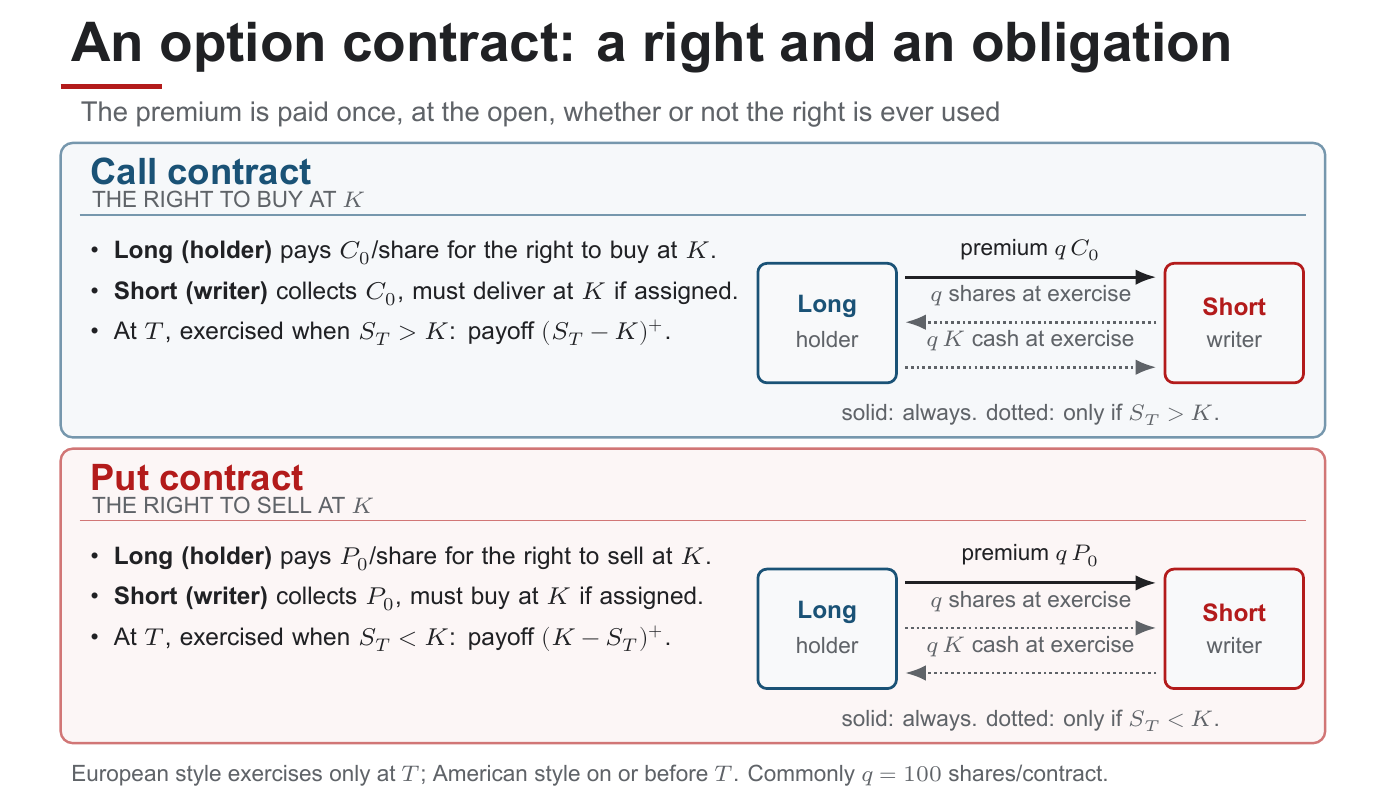
\includegraphics[width=0.66\textwidth,keepaspectratio]{../figs/Fig-L8b-Contract-Right-Obligation.png}
  \end{center}
  \vspace{-0.6em}
  One flow is unconditional, the premium at the open; two are conditional on
  exercise. \hilite{Long} positions risk only the premium, \hilite{short} ones
  collect it and carry the obligation.
\end{frame}

% ==== payoff =================================================
\begin{frame}{Expiration Payoff Is Contractual}
  For any real $x$ write $x^{+}\equiv\max(x,0)$. With $\ST\geq0$ the underlying
  price at expiration and $K>0$ the strike, both in USD/share, the payoff
  \hilite{per share} to the long holder is given by:
  \[
    \boxed{\hc(\ST;K)=\left(\ST-K\right)^{+},
      \qquad
      \hp(\ST;K)=\left(K-\ST\right)^{+}}
  \]
  The call holder exercises only when $\ST>K$, the put holder only when
  $\ST<K$, and otherwise abandons the right. Because the holder may always
  decline, \hilite{both payoffs are nonnegative}: the signature of a right.
  \begin{itemize}\setlength{\itemsep}{0.25em}
    \item \hilite{The short side mirrors it}: with direction
      $\theta\in\{-1,+1\}$, the signed payoff is $\theta\,\hc$ or $\theta\,\hp$.
    \item \hilite{Moneyness} classifies exercise value, not profit: a call is in
      the money when $\ST>K$, out of the money when $\ST<K$, and the put
      reverses these. It says nothing about whether the trade made money.
  \end{itemize}
\end{frame}

% ==== profit =================================================
\begin{frame}{Profit Requires a Cash-Flow Convention}
  Payoff belongs to the contract. \hilite{Profit belongs to the investor}, and it
  needs a rule for the premium, which moved at a different time. Under the
  \hilite{undiscounted convention}, with $C_0,P_0\geq0$ the premiums in USD/share
  and $\theta$ the direction, profit per share is given by:
  \[
    \boxed{\Pi_{T}^{\,c,\theta}(\ST)=\theta\Bigl(\underbrace{\hc(\ST;K)}_{\text{payoff at }T}-\underbrace{C_0}_{\text{premium at }0}\Bigr),
      \qquad
      \Pi_{T}^{\,p,\theta}(\ST)=\theta\Bigl(\hp(\ST;K)-P_0\Bigr)}
  \]
  For a long position the premium is an outflow, for a short an inflow: one
  $\theta$ multiplies both terms.
  \begin{itemize}\setlength{\itemsep}{0.25em}
    \item \hilite{Say what it hides}: this mixes time-$0$ and time-$T$ dollars,
      which every earlier lecture avoided. A time-$T$ P\&L would grow the
      premium forward, a time-$0$ value would discount the payoff (L1b).
    \item \hilite{Why use it}: it gets the shape and the breakeven right with the
      fewest moving parts. A convention, not an accounting identity.
  \end{itemize}
\end{frame}

\begin{frame}{Profit: Where a Position Breaks Even}
  The \hilite{breakeven} $S_{\mathrm{BE}}$, in USD/share, is the terminal price at
  which profit is exactly zero. Setting $\Pi_T=0$ on the exercised branch gives
  $\ST-K-C_0=0$ for the long call and $K-\ST-P_0=0$ for the long put, hence:
  \[
    \boxed{S_{\mathrm{BE}}^{\,c}=K+C_0,\qquad S_{\mathrm{BE}}^{\,p}=K-P_0}
  \]
  \begin{itemize}\setlength{\itemsep}{0.3em}
    \item \hilite{The breakeven is not the strike}: the premium shifts the curve
      down (long) or up (short) without moving the kink at $K$. On the AMD chain
      a $K=230$ call at $C_0=21.58$ breaks even at $251.58$: finishing in the
      money is not the same as making money.
    \item \hilite{Both directions share it}: short profit is the exact negative
      of long profit, so both sides agree on the breakeven price.
  \end{itemize}
  \slidenote{Example 1:}{\dimmed{CHEME-5660-L8b-Example-SingleContractPayoffProfit-Fall-2026.ipynb}}
\end{frame}

% ==== bounds =================================================
\begin{frame}{Loss Bounds and Direction Matter}
  \vspace{-0.2em}
  All per share; multiply by $q$ and by the number of contracts for account
  dollars.
  \vspace{0.3em}
  \begin{center}\small
  \begin{tabular}{@{}llll@{}}
    \textbf{\ink{Position}} & \textbf{\ink{Maximum profit}} & \textbf{\ink{Maximum loss}} & \textbf{\ink{Breakeven}}\\[2pt]
    \hline\\[-7pt]
    Long call  & unbounded as $\ST\to\infty$ & $C_0$ & $K+C_0$\\
    Short call & $C_0$ & unbounded as $\ST\to\infty$ & $K+C_0$\\
    Long put   & $K-P_0$ at $\ST=0$ & $P_0$ & $K-P_0$\\
    Short put  & $P_0$ & $K-P_0$ at $\ST=0$ & $K-P_0$\\
  \end{tabular}
  \end{center}
  \vspace{0.4em}
  The difference between the call rows and the put rows is the \hilite{domain}:
  $\ST\geq0$, so $\hp\leq K$ is capped by the strike, while $\hc$ has no cap
  because $\ST$ has none.
  \begin{itemize}\setlength{\itemsep}{0.2em}
    \item \hilite{Only one loss is genuinely unlimited}: the uncovered short
      call. The long call's profit is unbounded too, but no loss is.
    \item \hilite{A short put's loss is finite}: $K-P_0$ at $\ST=0$. On the
      $K=220$ contract collecting $16.33$, that is $203.67$ USD/share, or
      $20{,}367$ USD per contract. \hilite{Large is not unlimited}.
  \end{itemize}
\end{frame}

% ==== composite ==============================================
\begin{frame}{Composite Positions Add Leg by Leg}
  Let position $\CC$ contain legs $i=1,\ldots,d$ on one underlying and one
  expiration. Leg $i$ has strike $K_i>0$, direction $\theta_i\in\{-1,+1\}$,
  copies $n_i\in\N$, premium $P_i\geq0$ in USD/share, and long per-share payoff
  $h_i(\ST)$. The \hilite{per-share} totals are given by:
  \[
    \boxed{\HC(\ST)=\sum_{i=1}^{d}\underbrace{\theta_i\,n_i}_{\text{signed copies of leg }i}h_i(\ST),
      \qquad
      \PiC(\ST)=\sum_{i=1}^{d}\theta_in_i\bigl[h_i(\ST)-P_i\bigr]}
  \]
  \vspace{-0.9em}

  Both are in USD/share, which is what the example notebooks plot. For account
  dollars, multiply leg $i$ by its deliverable $q_i\in\N$ shares/contract.
  \begin{itemize}\setlength{\itemsep}{0.2em}
    \item \hilite{The kinks are the strikes}: each $h_i$ bends only at $K_i$, so
      the profit is piecewise linear, with a corner at strike $K$ exactly when
      the aggregate jump $\sum_{i:K_i=K}\theta_in_i$ is nonzero. Opposing legs
      at one strike cancel.
    \item \hilite{The offset is the net premium}: $\sum_i\theta_in_iP_i$, the
      net debit or credit, shifts the diagram without changing its shape.
  \end{itemize}
  Legs must share an underlying and an expiration for one diagram in $\ST$;
  deliverables may differ, so each $q_i$ is applied to its own leg.
\end{frame}

\begin{frame}{Composite Positions: Three Structures, One Sum}
  Three structures, $D$ the total premium per share:
  \begin{itemize}\setlength{\itemsep}{0.15em}
    \item \hilite{Vertical spread}: two legs of one type, different strikes,
      opposite directions. Both extremes finite.
    \item \hilite{Straddle}: a call and a put at one strike $K$, same direction.
      Profit $\theta\bigl(\lvert\ST-K\rvert-D\bigr)$, breakevens $K+D$ and,
      when $D\leq K$, $K-D$.
    \item \hilite{Strangle}: a call and a put at strikes $K_1<K_2$, same
      direction. A flat plateau replaces the straddle's single kink: a trough
      when long, a peak when short.
  \end{itemize}
  \textbf{\ink{State the bounds correctly.}} A long straddle is routinely said to
  have ``unlimited profit in either direction.'' \hilite{That is wrong on the
  downside.} Since $\ST\geq0$ the put leg cannot pay more than its strike, so the
  lower branch terminates: the AMD $K=230$ straddle with $D=42.88$ caps its
  downside at $187.12$ USD/share, while the upside has no bound.
  \slidenote{Example 2:}{\dimmed{CHEME-5660-L8b-Example-CompositeContractsPL-Fall-2026.ipynb}}
\end{frame}

% ==== optional advanced material =============================
\begin{frame}{Optional Advanced Material}
  \vspace{0.4em}
  {\normalsize\textbf{\ink{Advanced:}} \dimmed{advanced/static\_replication/}\par
  \dimmed{CHEME-5660-L8b-Advanced-Static-Replication-Fall-2026.ipynb}}

  \vspace{0.7em}
  Optional, not a prerequisite for L9a. The composite rule says adding legs
  \hilite{produces} payoff shapes; the notebook proves the converse. Every
  continuous piecewise-linear payoff with kinks $0<K_1<\cdots<K_d$ is
  $a+b\,\ST+\sum_i w_i(\ST-K_i)^{+}$ in \hilite{exactly one} way, with $a$ the
  payoff at zero, $b$ the initial slope, and $w_i$ the jump in slope at $K_i$. It
  proves existence by a telescoping sum of slopes and uniqueness by sweeping out
  from the leftmost interval, derives the put payoff identity, tabulates every
  structure above as one triple $(a,b,w)$, and marks the boundary of what a
  single expiration can reach.
  \slidenote{Notebook:}{\href{https://github.com/varnerlab/CHEME-5660-CourseRepository-Fall-2026/tree/main/lectures/week-8/L8b/advanced}{lectures/week-8/L8b/advanced}, also linked from the lecture notebook.}
\end{frame}

\begin{frame}{Summary}
  Today we translated contract terms into expiration cash flows and kept the
  contractual payoff separate from the investor's premium-dependent profit.

  {\large\textbf{\ink{Key takeaways}}}
  \begin{itemize}\setlength{\itemsep}{0.1em}
    \item \hilite{Payoff belongs to the contract}: a long call pays
      $(\ST-K)^{+}$ and a long put pays $(K-\ST)^{+}$ per share, and short
      positions reverse those flows exactly. Only $\ST$ is uncertain.
    \item \hilite{Profit needs a convention}: premium, financing time,
      deliverable $q$, fees, and direction $\theta$ all enter, so strike,
      moneyness, and breakeven are three different things.
    \item \hilite{Loss bounds are asymmetric, and only one side is unlimited}:
      the uncovered short call has no finite bound because $\ST$ has none; a
      standard short put's worst case is finite at $K-P_0$, reached at $\ST=0$.
  \end{itemize}
  Next, L9a values European claims with Black--Scholes--Merton and American
  claims with a Cox--Ross--Rubinstein lattice: where the premium comes from.
\end{frame}

\transitionframe{Today: what the contract promises, what the investor earns, and why only one of the four positions can lose without bound.}

\end{document}
